\begin{itemize}
    \item Ранее в билетах мы доказывали, что если у нас построен набор точек, то следующая построенная точка будет лежать в расширении степени не более 2. (Это следовало из того, что уравнение, задающее эту точку, имело степень не более 2).
    
    Расширение $K_i \supset K_{i+1}$ порождается одним элементом, то есть  $K_i = K_{i+1}(\gamma)$. По теореме о примитивном элементе (след. билет) есть неприводимый многочлен, корень которого порождает расширение, и его степень равна степени расширения, то есть не более 2.
    
    \item Если $z$ лежит в башне расширений, то нужно уметь строить корень из числа, а также произведение чисел и обратное к числу (последние два -- через теорему Фалеса).

    
    Построение корня:
    
    На прямой рядом отметим отрезки длины $x$ и $1$
    
    Полученный отрезок $AC$ поделим пополам. Проведем окружность с центром в этом отрезке, проходящую через один из его концов. Пусть точка $B$ лежит на отрезке $AC$, причем, $AB = 1, BC = x$, $D$ -- центр окружности.
    
    Проведем из точки $B$ перпендикуляр к $AC$, точку пересечения с окружностью обозначим за $E$. Из подобия треугольников $ABE, EBC$ получим, что дляна отрезка $EB$ равна $\sqrt{x}$.\\
    
    \begin{minipage}{0.4\textwidth}
        \centering
        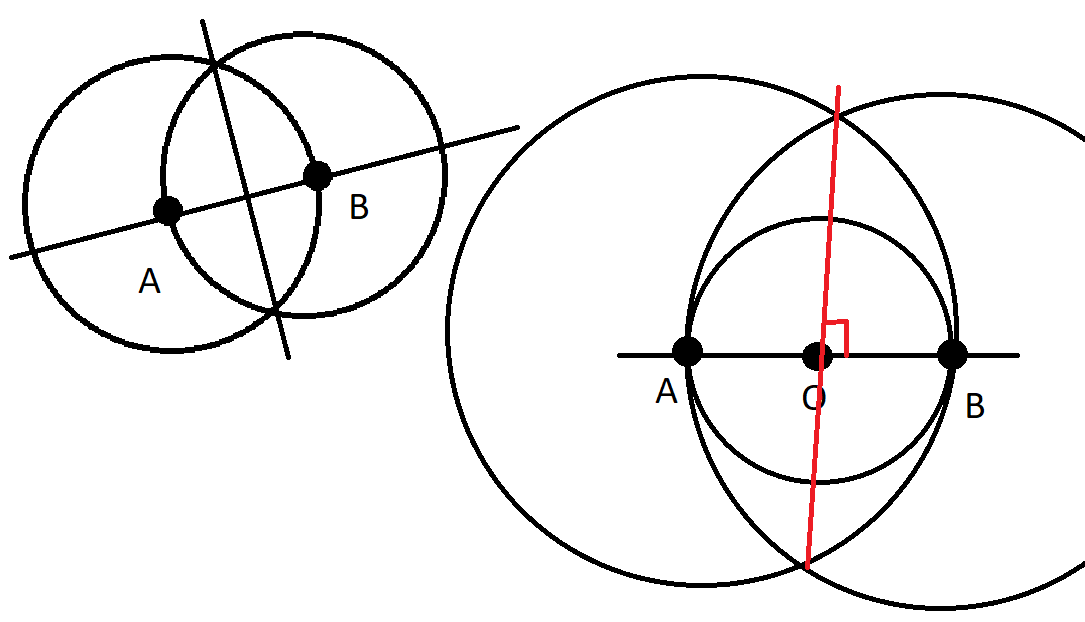
\includegraphics[width=0.7\linewidth]{sections/Ira/images/5-7_2.png}
    \end{minipage}\\
    
    На рисунке слева -- делим отрезок $AB$ пополам (проводя окружности с центром в одной точке и проходящие через другую).
    
    На рисунке справа -- восстанавливаем перпендикуляр из точки $O$. А именно сначала строим произвольную окружность с центром в точке $O$. Отмечаем точки пересечения с прямой $A, B$, а потом отрезок $AB$ <<делим пополам>>.
\end{itemize}